\chapter{PCA e Clustering}

\section{Traccia}
Dato un workload reale, trovarne uno sintetico e:

\begin{itemize}
    \item Trovare il miglior trade-off (numero di componenti principali e numero di cluster) tra perdita di devianza e diminuzione della dimensione dei dati.
    \item Discutere le differenze tra l'applicazione della clusterizzazione con e senza PCA.
\end{itemize}

\subsection{Raccolta dati}
I dati sono stati raccolti su un sistema con le caratteristiche mostrate in \cref{tab:pca_specs}.

\begin{table}[H]
\centering
    \begin{tabular}{|c|p{0.7\linewidth} |}
    \hline
    \multicolumn{1}{|c|}{\textbf{Caratteristiche}} &
    \multicolumn{1}{c|}{\textbf{Sistema}}  \tabularnewline \hline


CPU & AMD Ryzen 7, 5700U 1.8 GHz, 8 Core 16T L3 8MB \tabularnewline \hline

RAM & DDR4 SODIMM 16GB, 3200 MHz \tabularnewline \hline

OS & Linux-liquorix v6.6.1, 6.6.1-zen1-1-zen \tabularnewline \hline
\end{tabular}
\caption{Tabella riassuntiva delle caratteristiche del sistema}
\label{tab:pca_specs}
\end{table}

I dati sono stati raccolti leggendo una volta al secondo per $10$ minuti il \textit{file} \textbf{\textit{/proc/meminfo}} usando il \textit{benchmark} \textbf{nBody} eseguito $16$ volte per sfruttare tutte i \textit{core} del sistema (inclusi quelli virtuali).

Alla fine della misurazione, è stato ottenuto un \textit{dataset} composto da $600$ righe che descriverà il \textit{workload} iniziale.

\subsection{Pre-processing}
Rimosse le colonne con valori non numerici, si è proceduto a normalizzare i dati usando lo \textit{z-score}, trasformando il \textit{dataset} iniziale in uno a media zero e varianza unitaria, applicando la \cref{eq:zscore} per ogni parametro $s$.

\begin{equation}
    x'_s = \frac{x_s - \mu_s} {\sigma_s}
    \label{eq:zscore}
\end{equation}

 in cui con $\sigma_s$ e $\mu_s$ si indicano rispettivamente la deviazione standard a la media del parametro $s$.

 \subsection{Principal component analysis}
L'analisi a componenti principali è una tecnica che serve ad operare una trasformazione di stato. In particolare, il risultato della PCA è un nuovo dataset formato da colonne incorrelate ordinate in termini di variazione spiegata. Formalmente, detta $y_j$ la \textit{j-esima} componente principale, questa si definisce secondo la \cref{eq:pca}.

\begin{equation}
    y_j =  \mathlarger{\sum}_{i=1}^n w_{ij} x_{i}
    \label{eq:pca}
\end{equation}

Le tecniche utilizzate per implementare questo procedimento mirano a calcolare il peso $w_{ij}$.

Tuttavia, le componenti principali non hanno nessun significato fisico e quindi non possono essere utilizzate in sostituzione del dataset inziale per fare delle valutazioni. A valle della
PCA è inoltre possibile eliminare le componenti con variazione spiegata minore in modo da diminuire la dimensionalità del dataset.

\subsection{Clustering}
Il clustering è una tecnica che raggruppa elementi del dataset utilizzando una certa misura di distanza. È stata applicato il metodo di \textbf{\textit{Ward}} che mira a minimizzare la varianza \textit{intra-cluster} e massimizzare quella \textit{inter-cluster}. 

In particolar, la devianza intra-cluster si definisce come:
\begin{equation*}
    \mathlarger{\sum}_{k=1}^K \mathlarger{\sum}_{i=1}^{n_k} ||X_i - \overline{X}_k||^2
\end{equation*}

Invece, la devianza \textit{inter-cluster} è definita come:
\begin{equation*}
     \mathlarger{\sum}_{k=1}^K n_k ||\overline{X}_k - \overline{X}||^2
\end{equation*}

 
Dove si è ipotizzata la presenza di $K$ cluster, ciascuno dei quali con $n_k$ elementi e, per ogni cluster, viene calcolato il centroide con:
\begin{equation*}
    \overline{X}_k = \frac{1}{n_k} \mathlarger{\sum}_{i=1}^{n_k} X_i
\end{equation*}
 
In particolare, è stata applicata la tecnica del \textbf{clustering gerarchico agglomerativo} che, ad ogni iterazione, prevede la fusione di due cluster a distanza minima. 
 

 \subsection{Analisi}
 Per valutare la qualità del \textit{clustering} in termini di devianza persa, si è deciso di comparare l'effetto della scelta delle componenti post-PCA, variando il numero di componenti principali prima di effettuare il \textit{clustering}. In particolare, sarà effettuata una comparazione per $n \in (4, 8, 12)$, con $n$ è indicato il numero di componenti principali, e $m \in (10, 20, 30, 40)$ con $m$ numero di cluster. I risultati sono riportati in \cref{tab:pca_cl_comp}.

\begin{table}[H]
\centering
    \begin{tabular}{|c|c|c|c|c|c|}
    \hline
    \multicolumn{1}{|c|}{\textbf{N. PC}} &
    \multicolumn{1}{|c|}{\textbf{Devianza \%}} &
    \multicolumn{4}{|c|}{\textbf{Cluster}} \tabularnewline \hline

 &  & \textbf{10} & \textbf{20} & \textbf{30}  & \textbf{40} \tabularnewline \hline
\multirow{3}{*}{\textbf{4}} & Post PCA & $72.38$ & $72.38$ & $72.38$ & $72.38$ \\[1.25ex]
& Post Cluster & $64.52$ & $67.83$ & $69.08$ & $69.58$ \\ [1.25ex]
& Totale persa & $35.48$ & $32.17$ & $30.92$ & $30.42$

\tabularnewline \hline

\multirow{3}{*}{\textbf{8}} & Post PCA & $90.44$ & $90.44$ & $90.44$ & $90.44$ \\ [1.25ex] 
& Post Cluster & $64.66$ & $75.01$ & $78.32$ & $80.33$ \\ [1.25ex]
& Totale persa & $35.34$ & $24.99$ & $21.68$ & $19.67$ 

\tabularnewline \hline

\multirow{3}{*}{\textbf{12}} & Post PCA & $97.13$ & $97.13$ & $97.13$ & $97.13$ \\ [1.25ex]
& Post Cluster & $70.11$ & $78.75$ & $82.04$ & $84.12$ \\ [1.25ex]
& Totale persa & $29.89$ & $21.25$ & $17.96$ & $15.88$

\tabularnewline \hline

\end{tabular}
\caption{Risultati ottenuti facendo variare il numero di componenti principali e il numero di cluster}

\label{tab:pca_cl_comp}
\end{table}

Come si osserva in \cref{fig:pca_cluster_lost_dev}, gli effetti del numero di componenti principali sono più marcati all'aumentare del numero di cluster. Infatti, con $m=10$ tra $4$ e $8$ componenti la differenza è quasi nulla, mentre con $n=12$ abbiamo uno scarto del $5 \%$. Invece, con $m=40$ lo scarto tra $4$ e $12$ componenti principali diventa del $15\%$. Inoltre, si può osservare che con $n=8$ e $n=12$ la differenza in devianza persa rimane circa costante al variare del numero di cluster.

Ovviamente scegliere un numero elevato di componenti principali permette di diminuire la devianza persa inizialmente e di selezionare un numero minore di cluster. D'altro canto un numero elevato di componenti principali può appesantire il processo di \textit{clustering}.

\begin{figure}[H]
    \centering
    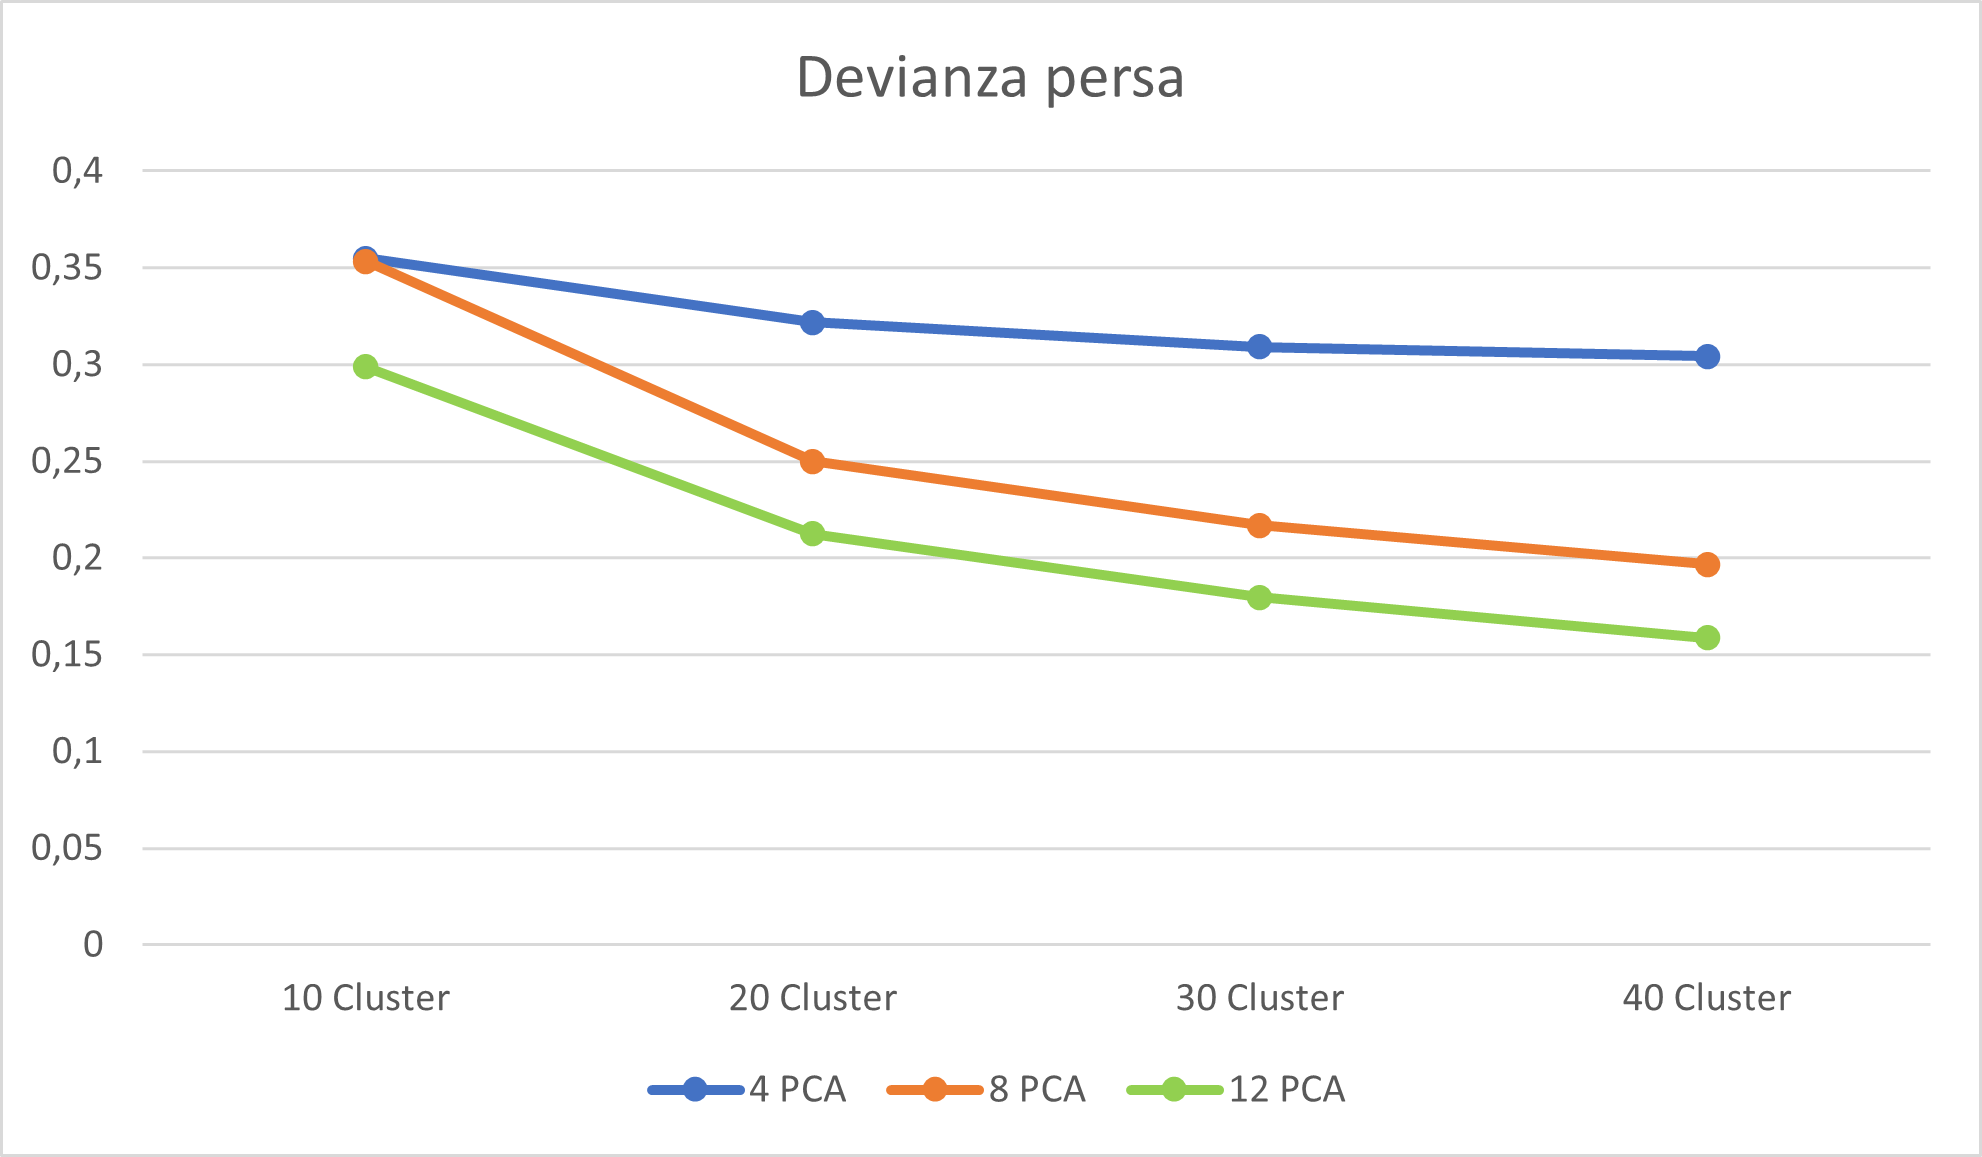
\includegraphics{img/ch2/lost_dev.png}
    \caption{Andamento devianza persa per numero di cluster e componenti principali}
    \label{fig:pca_cluster_lost_dev}
\end{figure}

\paragraph{Analisi outlier}Durante gli esperimenti si è notata la presenza di un
outlier corrispondente alla prima riga del dataset che nella magggior parte dei casi veniva assegnata ad un cluster isolato. Si è scelto di non scartare questa riga perchè ottenuta in condizioni di carico elevato.

\paragraph{Workload sintetico} Scegliendo $8$ componenti principali e $40$ cluster,
si è creato il workload sintetico (Figura \ref{fig:workload_synth}) con una devianza totale persa del $21.68\%$ con una
riduzione del dataset iniziale del $93.3\%$. L'elemento rappresentativo di ogni cluster è stato scelto randomicamente. 

\begin{figure}[H]
    \centering
    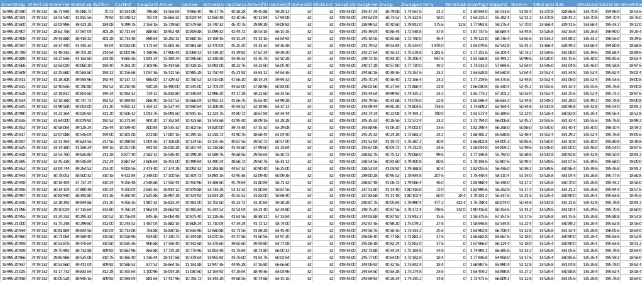
\includegraphics{img/ch2/synth_workload.png}
    \caption{Workload sintetico}
    \label{fig:workload_synth}
\end{figure}

